%%=============================================================================
%% Proof of Concept
%%=============================================================================

\chapter{\IfLanguageName{dutch}{Proof of Concept}{Proof of Concept}}%
\label{ch:proofofconcept}

\section{\IfLanguageName{dutch}{DLP Regels}{DLP Rules}}
\label{sec:DLP rules}

\subsection{\IfLanguageName{dutch}{Vooraf gedefinieerde regelsets}{Predefined Rulesets}}
\label{subsec:vooraf-gedefinieerde-regelsets}

In tabel \ref{tab:Netskope regelsets} staan de vooraf gedefinieerde regelsets van Netskope die zullen worden gebruikt in dit onderzoek. 
Deze regelsets moeten voldoen aan de Belgische en Europese wetgevingen, maar aangezien ze niet aanpasbaar zijn, zullen deze regelsets niet verder worden gepersonaliseerd. 
Mocht de vooraf gedefinieerde regelset niet voldoen aan de opgestelde evaluatiecriteria \ref{sec:correctheid}, dan zal er een nieuwe regelset worden gedefinieerd voor toekomstig gebruik. 
Deze nieuwe regelset zal een aanvullende rol krijgen om samen met de vooraf gedefinieerde regelsets te worden gebruikt.

\begin{table}[h]
    \centering
    \small
    \begin{tabular}{p{3cm}p{5cm}p{7cm}}
        \toprule
        \textbf{Wetgeving} & \textbf{Netskope Regelsets} & \textbf{Toelichting} \\
        \midrule
        AVG (GDPR) & 
        EU General Data Protection Regulation (GDPR) \newline 
        GDPR (narrow) & 
        Detectie van persoonsgegevens volgens de AVG. Narrow zal strikter en specifieker de gegevens detecteren. \\
        
        PCI DSS en DORA & 
        Payment Card Industry Data Security Standard. PCI-DSS \newline 
        DLP-PCI \newline 
        Best Practice PCI DLP Profile & 
        Detectie van creditcardgegevens, betalingsinformatie en andere financiële data. \\
        
        ISO 27001 & 
        Best Practice Confidential Tag Profile \newline 
        Best Practices ML-Based Detections & 
        Geen specifieke regelset, maar focus op governance, risicobeheer en vertrouwelijkheid. \\
        
        CCB-framework & 
        Best Practices ML-Based Detections & 
        Richtlijnen voor risicobeheer, gedragsanalyse en incidentdetectie via ML-gebaseerde detectie. \\
        
        NIS2 & 
        Custom policies + logging & 
        Richt op incidentdetectie en rapportering voor kritieke infrastructuur. \\
        \bottomrule
    \end{tabular}
    \caption{Mapping van wetgeving naar Netskope DLP-regelsets}
    \label{tab:Netskope regelsets}
\end{table}


\begin{table}[h]
    \centering
    \small
    \begin{tabular}{p{3cm}p{5cm}p{6cm}}
        \toprule
        \textbf{DLP-profiel} & \textbf{Gebruikte regels (predefined \& custom)} & \textbf{Toelichting / Doel} \\
        \midrule
        Persoonsgegevens Basis &
        EU-Identity-Name \newline
        EU-Name-DOB \newline
        EU-Name-Address \newline
        \textit{BE-National-ID (RRN)} &
        Basispakket voor identificatie van natuurlijke personen, inclusief Belgische RRN-detectie. Gericht op bredere AVG-compliance. \\
        
        Gevoelige gegevens &
        EU-Identity-Health \newline
        EU-Name-Religion \newline
        EU-Name-Race \newline
        EU-Name-Political \newline
        \textit{BE-HealthData-Tag} \newline
        \textit{BE-SocialeZekerheid} &
        Detectie van gevoelige data zoals gezondheid, religie, afkomst. Gericht op risico’s m.b.t. verwerking van bijzondere persoonsgegevens. \\
        
        Financiële gegevens &
        EU-Name-PAN \newline
        EU-Name-PAN-Exp \newline
        EU-Name-PAN-CVV \newline
        PCI-DSS \newline
        \textit{BE-IBAN, BE-BIC} &
        Beveiliging van betaal- en bankgegevens, met focus op DORA/PCI-DSS-compliance en Belgische bankstructuur. \\
        
        Overheidsdiensten &
        EU-Identity-Name \newline
        EU-Name-Region-Date \newline
        \textit{BE-Natinoal-ID (RRN)} \newline
        \textit{BE-NIS2-incidenten} \newline
        \textit{BE-FOD-Notificatieplicht} &
        Gericht op compliance voor openbare instellingen: incidentmelding, Belgische verplichtingen en gegevenslokalisatie. \\
        \bottomrule
    \end{tabular}
    \caption{Samengestelde DLP-profielen met gestructureerde weergave van regels}
    \label{tab:custom-dlp-profielen}
\end{table}


% Driver License: https://learn.microsoft.com/en-us/purview/sit-defn-belgium-drivers-license-number 


% Daarnaast stelt Netskope bedrijven in staat om maatwerk DLP-profielen te definiëren voor specifieke use-cases, 
% wat flexibiliteit biedt bij de bescherming van gevoelige gegevens. Netskope integreert ook compliance-informatie in zijn Cloud Confidence Index (CCI), 
% waarin het GDPR-nalevingsniveau van cloudapplicaties wordt aangegeven. 
% Hoewel Netskope geen actief filter biedt om automatisch maatregelen te nemen op basis van het GDPR-complianceniveau van een applicatie, 
% kunnen organisaties wel beveiligingsbeleid afstemmen op basis van de Cloud Index Score.

% Een beperking binnen de huidige regelsystemen is dat Netskope geen log bijhoudt van de fysieke locatie van een datacenter waarin een cloudapplicatie wordt gehost. 
% Hierdoor is het niet mogelijk om op basis hiervan specifieke beleidsregels af te dwingen. 
% Ook ontbreekt de functionaliteit om een blokkering of waarschuwing te genereren wanneer een gebruiker binnen een bepaalde periode een grote hoeveelheid data uploadt naar 
% een niet-goedgekeurde applicatie.


% Netskope biedt een uitgebreide set vooraf gedefinieerde regelsets binnen zijn Data Loss Prevention (DLP)-functionaliteit, 
% waarmee gevoelige informatie zoals Persoonlijk Identificeerbare Informatie (PII) effectief kan worden gedetecteerd en beschermd. 
% Volgens \textcite{brouwer2021cloud} heeft Netskope een uitgebreide lijst van DLP-profielen ontwikkeld die helpen bij het identificeren van verschillende soorten PII, 
% variërend van EU-identificatiegegevens tot Singaporese identificatiegegevens en medische rapporten. 
% De DLP-profielen van Netskope zijn goed uitgebalanceerd en sluiten aan bij de regelgeving van de meeste westerse landen.

% Naast deze vooraf gedefinieerde regels biedt Netskope de mogelijkheid om maatwerk DLP-profielen te definiëren voor specifieke use-cases. 
% Verder integreert Netskope compliance-informatie in zijn Cloud Confidence Index (CCI), waarin het GDPR-nalevingsniveau van cloudapplicaties wordt aangegeven. 
% Echter, zoals \textcite{brouwer2021cloud} opmerkt, biedt Netskope geen filter om automatisch maatregelen te nemen op basis van het GDPR-complianceniveau van een applicatie.

% Daarnaast houdt Netskope geen log bij van de fysieke locatie van een datacenter waarin een cloudapplicatie wordt gehost,
%  waardoor beleid op basis van datacenterlocatie niet kan worden afgedwongen. 
%  Ook merkt \textcite{brouwer2021cloud} op dat Netskope niet de mogelijkheid biedt om een waarschuwing of blokkade te genereren wanneer een gebruiker binnen een 
%  bepaalde periode een grote hoeveelheid data uploadt naar een niet-goedgekeurde applicatie.


% Netskope allows for identification of PII with the use of DLP.
% They have defined a comprehensive list of profiles to assist in
% detecting various kinds of PII e.g. EU Identification to Singapore
% Identification as well as medical reports. Netskope has well balanced
% DLP profiles serving most western countries. Additionally, it is
% also possible to define custom DLP profiles for specific use cases.
% Netskope defines the GDPR level a cloud application offers in its
% Cloud Confidence Index but does not offer a filter to define an
% action based on users visiting an app that does not meet a set
% GDPR compliance level. Netskope does not keep a record of the
% data center an application uses and can therefore not meet this use
% case requirement. The ability to define a filter based on the overall
% Cloud Index score is possible. Lastly, it is not possible to generate
% an alert or block action if a user uploads an X amount of data within
% a certain period of time to an unsanctioned application

\subsection{\IfLanguageName{dutch}{Aangepaste regelsets}{Custom Rulesets}}
\label{subsec:poc-aangepaste-regelsets}

% <https://docs.netskope.com/en/category-definitions/> \textcite{NetskopeCatDef2025}

Dit onderzoek bevat vooral aangepaste regels, ontwikkeld om aan de specifieke behoeften van de organisatie te voldoen. 
De regels die nog niet bij Netskope zijn gedefinieerd en ontwikkeld op basis van een combinatie van vooraf gedefinieerde regels, eigen woordenlijsten en reguliere expressies. 
Elke gemaakte DLP-regel bevat volgende elementen:


{\small
\begin{itemize}
    \item \textbf{Regel}: De naam van de DLP-regel die wordt gebruikt.
    \item \textbf{Type}: Het type DLP-regel dat wordt gebruikt. Dit kan een DLP regel zijn of een fingerprint.
    \item \textbf{Expressie}: De expressie die wordt gebruikt om de DLP-regel te definiëren. P staat voor 'predefined', D staat voor 'custom dictionary' en E voor 'exact match'.
    \item \textbf{\textit{Predefined Identifiers}}: De vooraf gedefinieerde entiteiten die worden gebruikt in de expressie. Dit zijn entiteiten die door Netskope zijn gedefinieerd en die kunnen worden gebruikt in de DLP-regel.
    \item \textbf{\textit{Custom Dictionary Identifiers}}: De aangepaste entiteiten die worden gebruikt in de expressie. Hierin staan lijsten van woorden, nummers of reguliere expressies gedefinieerd. 
    \item \textbf{\textit{RegEx}}: De reguliere expressies die worden gebruikt in de DLP-regel, zoals bijvoorbeeld voor het rijksregisternummer.
    \item \textbf{\textit{Exact match}}: De exacte match die wordt gebruikt om de DLP-regel te definiëren. 
    \item \textbf{Gebruikte techniek}: De techniek die wordt gebruikt om de DLP-regel te definiëren.
    \item \textbf{\textit{Bron(nen)}}: De bronnen die zijn gebruikt om de DLP-regel te definiëren. Dit kunnen woordenlijsten zijn, maar ook andere bronnen zoals websites of documenten.
    \item \textbf{Threshold}: De drempelwaarde die wordt gebruikt om de DLP-regel te definiëren. Dit kan 'Low', 'Medium', 'High' of 'Critical' zijn. Vanaf de waarde 'Medium' zal Netskope de actie van de gebruiker blokkeren. 'Low' is enkel een waarschuwing.
\end{itemize}
}

In tabellen \ref{tab:custom-be-id}, \ref{tab:custom-be-iban} en \ref{tab:custom-be-iban-terms}, \ref{tab:custom-eu-card} en \ref{tab:custom-eu-card-terms} staan de aangepaste DLP-regels die zijn ontwikkeld voor dit onderzoek. 
Dankzij het gebruik van DLP-regels met en zonder termen, kunnen false positives sneller worden gedetecteerd. 
\textbf{Meer regels worden hier nog aan toegevoegd, momenteel moeten ze nog getweaked worden.}

\begin{table}[h]
    \centering
    \small
    \begin{tabular}{p{4cm} p{10cm}}
        \toprule
        \textbf{Regel} & BE - National ID and Surname \\
        \midrule
        \textbf{Type} & DLP Rule \\
        \textbf{Expressie} & \texttt{(P1 OR P2) AND (P0 OR D0 OR D1)} \\
        \textbf{Predefined Identifiers} & 
        (P0) - Surnames (International) \newline
        (P1) - National ID Numbers (BE) \newline
        (P2) - National ID Terms (BE; “RRN”) \\
        \textbf{Custom Dictionary Identifiers} & 
        (D0) - Full Names (BE) A-P \newline
        (D1) - Full Names (BE) P-Z \\
        \textbf{Gebruikte techniek} & Regex voor RRN in combinatie met woordenlijsten van Belgische achternamen \\
        \textbf{Bron(nen)} & \textcite{Statbel2023, Statbel2024} \\
        \textbf{Threshold} & Low: 2 \quad Medium: 10 \quad High: 25 \quad Critical: 50 \\
        % \textbf{Extra} & OBFUSCATION? https://docs.netskope.com/en/dlp-entity/#:~:text=Entities%20are%20used%20in%20a,click%20on%20the%20Entities%20tab. \\
        \bottomrule
    \end{tabular}
    \caption{Custom DLP-regel: Detectie van Belgische rijksregisternummers in combinatie met familienamen}
    \label{tab:custom-be-id}
\end{table}



\begin{table}[h]
    \centering
    \small
    \begin{tabular}{p{4cm} p{10cm}}
        \toprule
        \textbf{Regel} & BE -  \\
        \midrule
        \textbf{Type} & DLP Rule \\
        \textbf{Expressie} & \texttt{} \\
        \textbf{Predefined Identifiers} & 
        (P0) - \newline
        (P1) - \newline
        (P2) -  \\
        \textbf{Custom Dictionary Identifiers} & 
        (D0) - \newline
        (D1) - \\
        \textbf{Gebruikte techniek} & \\
        \textbf{Bron(nen)} & \textcite{} \\
        \textbf{Threshold} & Low: 2 \quad Medium: 10 \quad High: 25 \quad Critical: 50 \\
        \bottomrule
    \end{tabular}
    \caption{Custom DLP-regel: }
    \label{tab:custom-}
\end{table}


\begin{table}[h]
    \centering
    \small
    \begin{tabular}{p{4cm} p{10cm}}
        \toprule
        \textbf{Regel} & BE - PCI - IBAN \\
        \midrule
        \textbf{Type} & DLP Rule \\
        \textbf{Expressie} & \texttt{P0 OR P1 OR P2 OR P3 } \\
        \textbf{Predefined Identifiers} & 
        (P0) - Deposit Account Numbers (BE)
        (P1) - IBAN (BE; formatted)
        (P2) - IBAN (BE; unformatted)
        (P3) - IBAN (all) \\
        \textbf{Gebruikte techniek} & Vooraf gedefinieerde DLP identifiers gebruikt rond IBAN en bankrekeningnummers \\
        \textbf{Bron(nen)} & Null \\
        \textbf{Threshold} & Low: 1 \quad Medium: 3 \quad High: 5 \quad Critical: 10 \\
        \bottomrule
    \end{tabular}
    \caption{Custom DLP-regel: }
    \label{tab:custom-be-iban}
\end{table}

\begin{table}[h]
    \centering
    \small
    \begin{tabular}{p{4cm} p{10cm}}
        \toprule
        \textbf{Regel} & BE - PCI - IBAN with Bank Terms \\
        \midrule
        \textbf{Type} & DLP Rule \\
        \textbf{Expressie} & \texttt{(P2 NEAR P0) OR (P2 NEAR P1) OR (P2 NEAR P6) OR (P2 NEAR P7) OR (P2 NEAR P8) OR (P3 NEAR P0) OR (P3 NEAR P1) OR (P3 NEAR P6) OR (P3 NEAR P7) OR (P3 NEAR P8) OR (P4 NEAR P0) OR (P4 NEAR P1) OR (P4 NEAR P6) OR (P4 NEAR P7) OR (P4 NEAR P8) OR (P5 NEAR P0) OR (P5 NEAR P1) OR (P5 NEAR P6) OR (P5 NEAR P7) OR (P5 NEAR P8)} \\
        \textbf{Predefined Identifiers} & 
        (P0) - IBAN Terms \newline 
        (P1) - Bank Account Terms (BE) \newline
        (P2) - Deposit Account Numbers (BE) \newline
        (P3) - IBAN (BE; formatted) \newline
        (P4) - IBAN (BE; unformatted) \newline
        (P5) - IBAN (all) \newline
        (P6) - Card Number Terms (English) \newline
        (P7) - Card Security Terms (English) \newline
        (P8) - Bank Account Number Terms (English) \\
        \textbf{Gebruikte techniek} & Vooraf gedefinieerde DLP identifiers gebruikt rond IBAN en bankrekeningnummers in combinatie met woordenlijsten van Belgische termen. \\
        \textbf{Bron(nen)} & Null \\
        \textbf{Threshold} & Low: 1 \quad Medium: 2 \quad High: 5 \quad Critical: 9 \\
        \bottomrule
    \end{tabular}
    \caption{Vooraf gedefinieerde DLP-regel: Detectie van Belgische IBAN-nummers in combinatie met banktermen}
    \label{tab:custom-be-iban-terms}
\end{table}



\subsection{\IfLanguageName{dutch}{Persoonlijke gegevens (PII)}{Personal Data}}
\label{subsubsec:Persoonlijke gegevens}

\subsubsection{\IfLanguageName{dutch}{Identificatiegerichte regels}{Identification Rules}}
\label{subsubsec:identificatiegerichte-regels}

\subsubsection{\IfLanguageName{dutch}{Gevoelige persoonsgegevens}{Sensitive Personal Data}}
\label{subsubsec:gevoelige-persoonsgegevens}



\subsection{\IfLanguageName{dutch}{Betalingsgegevens (PCI)}{Financial Data}}
\label{subsubsec:betalingsgegevens}

% \subsubsection{\IfLanguageName{dutch}{)}{}}
% \label{subsubsec:}

https://www.b2bpay.co/list-banks-europe



\section{\IfLanguageName{dutch}{Toepassingen}{Applications}}
\label{subsubsec:toepassingen}

Tabel \ref{tab:toepassingen} geeft een overzicht van de gemaakte profielen 
Dit zijn toepassingen van de eerder opgestelde regels in Tabel \ref{tab:datatypes_risico}.


\begin{table}[h]
    \centering
    \small
    \begin{tabular}{p{3cm}p{5cm}p{6cm}}
        \toprule
        \textbf{Toepassing} & \textbf{Categorieën (Netskope)} & \textbf{Voorbeelden van applicaties} \\
        \midrule
        \textbf{SaaS}     & Collaboration, Cloud Storage, Application Suite & Slack, Teams, Teamleader, Google Drive, Jira, Confluence \\
        \textbf{Web}      & Professional Networking, Development Tools & LinkedIn, GitHub \\
        \textbf{IaaS}     & \gls{iaas}/\gls{paas}, Web Hosting, \gls{isp} & AWS, Azure, Google Cloud, OVH, DigitalOcean, Cloudflare \\
        \textbf{Email}    & Webmail, Email Outbound App & Gmail, Outlook, ProtonMail, Mailchimp, Thunderbird \\
        \textbf{Endpoint} & Endpoint DLP, Utilities & \gls{usb}, clipboard, printers, external devices \\
        \bottomrule
    \end{tabular}
    \caption{Overzicht van de verschillende toepassingen van de DLP-regels}
    \label{tab:toepassingen}
\end{table}



\subsection{\IfLanguageName{dutch}{Software as a Service (SaaS)}{Software as a Service (SaaS)}}
\label{subsubsec:saas-poc}
% Forward proxy and API 
% Slack, Teams, Teamleader, Google Drive, Jira, Confluence
% \textbf{Hierin komt er een overzicht van hoe SaaS toepassingen werken met Netskope. en hoe ik deze heb geimplenteerd.}

% In de SaaS-omgeving werd de focus gelegd op het beveiligen van cloudapplicaties zoals Slack, 
% Microsoft Teams, Google Drive, Jira en Confluence. Deze applicaties vallen onder de categorieën Collaboration en Cloud Storage. 
% Door gebruik te maken van een forward proxy via de Netskope Client en API-integraties met deze diensten, 
% werd zowel Data-in-Motion als Data-at-Rest beschermd. 
% Via de API werden bestanden gescand op gevoelige informatie op het moment van upload, synchronisatie of delen. 
% Door middel van policyregels gebaseerd op GDPR- en PCI-profielen werd onder andere het delen van persoonsgegevens en creditcardinformatie geblokkeerd of gelogd.

In de SaaS-omgeving worden cloudapplicaties zoals \textbf{\textit{Slack}}, \textbf{\textit{Microsoft Teams}}, \textbf{\textit{Teamleader}}, 
\textbf{\textit{Google Drive}}, \textbf{\textit{Jira}} en \textbf{\textit{Confluence}} beveiligd door een combinatie van forward proxy-verkeer en geavanceerde API-integraties binnen Netskope. 
Deze toepassingen \ref{tab:toepassingen} vallen onder de categorieën \textit{Collaboration}, \textit{Cloud Storage} en \textit{Application Suite} \autocite{Netskope2025API}.

De \textit{\textbf{forward proxy}}-setup zorgt voor real-time controle over gebruikersverkeer, 
inclusief het scannen van bestanden en berichten tijdens het verzenden of uploaden. 
Hierdoor wordt data-in-motion onmiddellijk geanalyseerd en geblokkeerd indien nodig.

Via API-integraties worden bestanden en berichten gescand op het moment van upload, synchronisatie of delen \autocite{Netskope2025API}. 
Zo wordt ook data-at-rest beschermd, bijvoorbeeld bij reeds opgeslagen documenten in Google Drive of bij gedeelde bestanden in Slack-kanalen \autocite{Netskope2022Slack}.

De integraties van deze applicaties met Netskope zijn deels al geïmplementeerd door Evolane. 
Aangezien de focus van dit onderzoek ligt op de DLP-regels, zal deze integratie niet verder uitgewerkt worden.

\subsection{\IfLanguageName{dutch}{Web}{Web}}
\label{subsubsec:web-poc}
% Forward proxy hiermee 
% LinkedIn, Github

In de webomgeving wordt uitgaand verkeer beveiligd via een forward proxy in combinatie met SSL-inspectie. 
Netskope onderschept versleutelde HTTPS-verzoeken en analyseert deze op de aanwezigheid van confidentiële data.
Zo wordt het dataverlies via webformulieren, berichten of uploads proactief tegengehouden. 
Deze aanpak focust op \textit{data-in-motion} en wordt toegepast op websites zoals \textbf{LinkedIn}, \textbf{GitHub}, \textbf{Messenger}, \textbf{ChatGPT} en \textbf{Google Forms}.

Om deze functionaliteit te testen, wordt gebruikt gemaakt van een dataset met realistische testwaarden. 
De testdata bevatte combinaties van persoonsnamen, en creditcardnummers (\textit{Visa} en \textit{Mastercard}), gestructureerd in \gls{csv}-formaat. Enkele voorbeelden:

\begin{quote}\small
\texttt{Robert Aragon, 4929-3813-3266-4295} \
\texttt{Ashley Borden, 5370-4638-8881-3020}
\end{quote}

Voor deze evaluatie werd een Python-script opgebouwd dat gebruikmaakt van Selenium. 
Het script is ontworpen om testgegevens aan de hand van batches in te voeren via het online platform \texttt{dlptoolbox.com}.
Dit platform biedt een veilige manier om DLP-regels realistisch te testen binnen de browseromgeving van de gebruiker.
Het script stuurt gegevens automatisch in batches van tien rijen naar het testformulier \ref{lst:dlp-selenium} en verzendt deze data aan de hand van een \texttt{POST}-request naar de server.
Dit werd tijdens de evaluatie in rijen van 10 gedaan, aangezien de testgegevens \ref{tab:csv-testdata} 30 000 rijen bevatten.

{\small
\begin{lstlisting}[language=Python,caption={Versturen van batches via Selenium},label={lst:dlp-selenium}, captionpos=b, basicstyle=\small\ttfamily]
from selenium.webdriver.common.by import By
from selenium.webdriver.support import expected_conditions as EC
textarea = wait.until(EC.presence_of_element_located((By.ID, "clientDataClear")))
textarea.clear()
textarea.send_keys(batch)
\end{lstlisting}
}


Na verzending wordt de gelekte data teruggelezen en geëvalueerd \ref{lst:dlp-teruggelezen}. Netskope staat in alert modus, zodat alle keren dat er gevoelige data wordt gedetecteerd, een incident wordt aangemaakt. 

{\small
\begin{lstlisting}[language=Python, caption={Versturen van batches via Selenium},label={lst:dlp-teruggelezen}, captionpos=b, basicstyle=\small\ttfamily]
leaked_box = driver.find_element(By.ID, "clientDataLeaked")
leaked_data = leaked_box.get_attribute("value")
print(f"Gelekte data:\n{leaked_data}")
\end{lstlisting}
}

Elke testcyclus werd afgesloten met een reset van het formulier om interferentie te voorkomen. 
Elk incident werd gelogd op Netskope en zal in Hoofdstuk \ref{ch:resultaten} verder worden besproken.

% \begin{lstlisting}[language=Python,label={lst:dlp-selenium},caption={Selenium-script voor batchgewijze verzending van testdata}]
%     code hier
% \end{lstlisting}

% \begin{lstlisting}[style=custompython,caption={Selenium-script voor batchgewijze verzending van testdata},label={lst:dlp-selenium}]
%     from selenium import webdriver
%     from selenium.webdriver.common.by import By
%     from selenium.webdriver.chrome.options import Options
%     from selenium.webdriver.support.ui import WebDriverWait
%     from selenium.webdriver.support import expected_conditions as EC
%     import time
    
%     # Config
%     URL = "https://dlptoolbox.com/postmaster.aspx"
%     INPUT_FILE = "dlp_testdata.csv"
%     ROWS_PER_BATCH = 10
%     WAIT_SECONDS = 5
    
%     # Setup Chrome
%     options = Options()
%     options.add_argument("--headless")
%     driver = webdriver.Chrome(options=options)
%     wait = WebDriverWait(driver, 10)
    
%     driver.get(URL)
%     iframe = wait.until(EC.presence_of_element_located((By.ID, "ifrPOST")))
%     driver.switch_to.frame(iframe)
    
%     with open(INPUT_FILE, 'r') as f:
%         lines = [line.strip() for line in f if line.strip()]
    
%     for i in range(0, len(lines), ROWS_PER_BATCH):
%         batch = "\n".join(lines[i:i+ROWS_PER_BATCH])
%         print(f"📤 Versturen batch {i//ROWS_PER_BATCH + 1}:\n{batch} 📤")
    
%         textarea = wait.until(EC.presence_of_element_located((By.ID, "clientDataClear")))
%         textarea.clear()
%         textarea.send_keys(batch)
    
%         launch_btn = wait.until(EC.element_to_be_clickable((By.ID, "btnLaunch")))
%         launch_btn.click()
%         time.sleep(WAIT_SECONDS)
    
%         leaked_box = driver.find_element(By.ID, "clientDataLeaked")
%         leaked_data = leaked_box.get_attribute("value")
%         print(f"Gelekte data ({len(leaked_data)} tekens):\n{leaked_data}")
%         print("—" * 50)
    
%         try:
%             reset_btn = wait.until(EC.element_to_be_clickable((By.ID, "btnReset")))
%             reset_btn.click()
%             time.sleep(1)
%         except Exception as e:
%             print(f"[!] Reset mislukt: {e}")
    
%     driver.quit()
% \end{lstlisting}
    

\subsection{\IfLanguageName{dutch}{Infrastructure as a Service (IaaS)}{Infrastructure as a Service (IaaS)}}
\label{subsubsec:iaas-poc}
% Forward proxy and API
% Linode, Akamai, AWS, Azure, Google Cloud, Digital Ocean, OVH, Vultr, Hetzner, Kinsta, Cloudflare,

In de IaaS-omgeving biedt Netskope beveiliging aan de hand van forward proxy en API-integraties. 
Platforms zoals \textbf{\textit{AWS}}, \textbf{\textit{Azure}}, \textbf{\textit{Google Cloud}}, \textbf{\textit{DigitalOcean}}, \textbf{\textit{OVH}}, \textbf{\textit{Hetzner}}, \textbf{\textit{Linode}} 
en \textbf{\textit{Cloudflare}} vallen onder deze categorie. Deze cloudinfrastructuurplatforms worden vaak gebruikt voor het hosten van virtuele machines, opslagdiensten en netwerkcomponenten.

% De IaaS-toepassingen omvatten onder andere AWS, Azure en Google Cloud. 
% Zowel API-gebaseerde scanning van opslag (zoals S3-buckets) als realtime monitoring via proxies werden onderzocht. 
% In deze omgeving werd gecontroleerd op het onbedoeld delen van gevoelige bestanden of configuraties, 
% zoals exports van databases met persoonsgegevens. Met behulp van aangepaste DLP-profielen werd onder meer detectie uitgevoerd op Belgische identiteitsnummers en medische gegevens. 
% Incidentmeldingen werden gelogd conform de NIS2-verplichtingen.




\subsection{\IfLanguageName{dutch}{Email}{Email}}
\label{subsubsec:email-poc}
% Webmail and API
% Outlook, Gmail, Exchange, Office 365, Thunderbird, Protonmail, Mailchimp, Sendinblue



% Voor e-mailverkeer werd DLP toegepast op zowel webmail (zoals Gmail, Outlook Web Access) als traditionele clients (Thunderbird, Outlook). 
% Netskope detecteerde en blokkeerde gevoelige bijlagen of tekstinhoud vóór verzending (outbound). 
% Via API-integraties met Microsoft 365 en Gmail konden berichten en bijlagen worden gescand op basis van GDPR-regels, 
% PCI-gegevens en Belgische identifiers (zoals RRN of sociale zekerheid). Zo werd voorkomen dat vertrouwelijke informatie onbedoeld via e-mail naar onbevoegde ontvangers werd verzonden.




\subsection{\IfLanguageName{dutch}{Endpoint}{Endpoint}}
\label{subsubsec:endpoint-poc}
% Endpoint DLP
% USB, clipboard, printers, external devices

% Op endpoints werd DLP geïmplementeerd via de Netskope Client. 
% De focus lag op het beveiligen van Data-in-Use. 
% Dit omvatte monitoring van kopieeracties naar USB-opslag, 
% gebruik van het klembord (clipboard), en het printen van gevoelige documenten. 
% In geval van een policyovertreding, zoals het kopiëren van een bestand met gevoelige persoonsgegevens naar een extern apparaat, 
% werd een waarschuwing getoond of de actie geblokkeerd. Daarnaast werd gecontroleerd of data buiten het bedrijfsnetwerk werd verplaatst zonder encryptie.





% In dit onderzoek wordt een Proof of Concept (PoC) klantomgeving ontwikkeld voor Evolane. 
% In deze omgeving worden zowel confidentiële als niet-confidentiële gegevens verwerkt en opgeslagen. 
% Door een Data Leakage Prevention-oplossing te implementeren, worden deze gegevens beveiligd tegen lekken. De DLP-oplossing moet voldoen aan de Belgische wetgeving, 
% waaronder de Algemene Verordening Gegevensbescherming (AVG) over persoonsgegevens (PII) en de Payment Card Industry Data Security Standards (PCI DSS) met betrekking tot betalingsgegevens (PCI). 
% De DLP-oplossing moet verder rekening houden met de NIS2-richtlijn en andere cybersecuritykaders, zoals het CCB-kader of ISO 27001. 
% De PoC bevat een Netskope-gebaseerde DLP-oplossing die confidentiële gegevens beschermt en voldoet aan de Belgische regelgeving. 

% Om een breder inzicht te verkrijgen in de implementatie en optimalisatie van Data Loss Prevention (DLP)-oplossingen, wordt in deze bachelorproef verder onderzocht hoe DLP kan worden toegepast in verschillende contexten en omgevingen. De onderstaande gebieden vormen de focus van dit onderzoek:

% \begin{itemize}
% \item \textbf{SaaS} (Software as a Service): DLP-oplossingen richten zich op gegevens in beweging (\textit{Data-in-Motion}), zoals bij het gebruik van forward proxies en bij statische gegevens (\textit{Data-at-Rest}) voor APIs.
% \item \textbf{Web}: Hier wordt DLP toegepast op geëncrypteerd verkeer en voor alle poorten, met focus op gegevens in beweging tussen systemen.
% \item \textbf{IaaS} (Infrastructure as a Service): Net zoals bij SaaS, wordt DLP toegepast op gegevens in beweging en in rust, ook 
% \item \textbf{Email}: Bij het beheren van e-mailverkeer, zoals webmail, richt de uitgewerkte DLP-oplossing zich zowel op gegevens in beweging als op gegevens in rust.
% \item \textbf{Endpoint}: Endpoint Data Loss Prevention (DLP) richt zich op het beschermen van gegevens in gebruik (\textit{Data-in-Use}) door middel van endpointbeveiliging. Dit houdt het volgende in: het monitoren en beperken van gegevensoverdracht via USB-opslagmedia, klemborden, printers en andere externe apparaten.
% \end{itemize}

\section{\IfLanguageName{dutch}{Automatisering van Gegevensverwerking en Testverkeer}{Automation of Data Processing and Test Traffic}}
\label{sec:automatisering-poc}

% Om de DLP-regels te testen werd een Python-script ontwikkeld dat een lokaal Flask-webformulier draait en dit via ngrok publiek toegankelijk stelt \autocite{ngrok2025}. 
% Een Selenium WebDriver bestuurt vervolgens een browser om gebruikersgedrag te simuleren. Het script vult het formulier in met \textt{textarea.send_keys(..)} \ref{lst:ngrok-textarea}
% en verstuurt de gegevens naar de server met \textt{element.click()} \ref{lst:ngrok-click} \autocite{Selenium2025ActionChains, Selenium2025WebDriver}.
% \textcite{Parmar2024} legde kort de basis uit van hoe Selenium werkt en hoe het kan worden gebruikt om een webbrowser te automatiseren.
% Deze aanpak is terug te vinden in de codefragmenten  

% Selenium2025ActionChains   Selenium2025WebDriver   Parmar2024

% {\small
% \begin{lstlisting}[language=Python,caption={textarea_send_key},label={lst:ngrok-textarea}, captionpos=b, basicstyle=\small\ttfamily]
% def try_send(email_content):
% for attempt in range(RETRY_LIMIT + 1):
%     try:
%         textarea = wait.until(EC.presence_of_element_located((By.ID, "sensitive_data")))
%         textarea.clear()
%         try:
%             textarea.send_keys(email_content)
%         except Exception:
%             actions = ActionChains(driver)
%             actions.move_to_element(textarea).click().send_keys(email_content)
%             actions.perform()
% \end{lstlisting}
% }

% {\small
% \begin{lstlisting}[language=Python,caption={element_click},label={lst:ngrok-click}, captionpos=b, basicstyle=\small\ttfamily]
% WebDriverWait(driver, 5).until(
%     EC.presence_of_element_located((By.ID, "result"))
% )
% \end{lstlisting}
% }


% In het kader van deze Proof of Concept werd een aangepaste automatisatiepijplijn ontwikkeld om testdata efficiënt en gecontroleerd aan een Data Loss Prevention (DLP)-systeem aan te bieden. 
% Hiervoor werd gekozen om gebruik te maken van Selenium WebDriver in combinatie met een lokale webapplicatie die tijdelijk toegankelijk werd gemaakt via Ngrok. 
% Selenium bood de flexibiliteit om menselijke interactie met de webinterface na te bootsen, wat essentieel was voor het correct simuleren van gebruikersgedrag zonder manuele tussenkomst. 
% Ngrok werd gekozen om de applicatie die lokaal draait tijdelijk en veilig publiek beschikbaar te maken, zonder extra netwerkinfrastructuur of firewall-aanpassingen. 
% Door testdata automatisch te injecteren in de webinterface en bijhorende response-informatie te verzamelen, 
% werd een schaalbare en reproduceerbare testomgeving opgezet voor de evaluatie van verschillende DLP-regels en detectielogica.

\section{\IfLanguageName{dutch}{Netskope alerts}{Netskope alerts}}
\label{subsubsec:netskope-alerts}

% \begin{figure}[h]
%     \centering
%     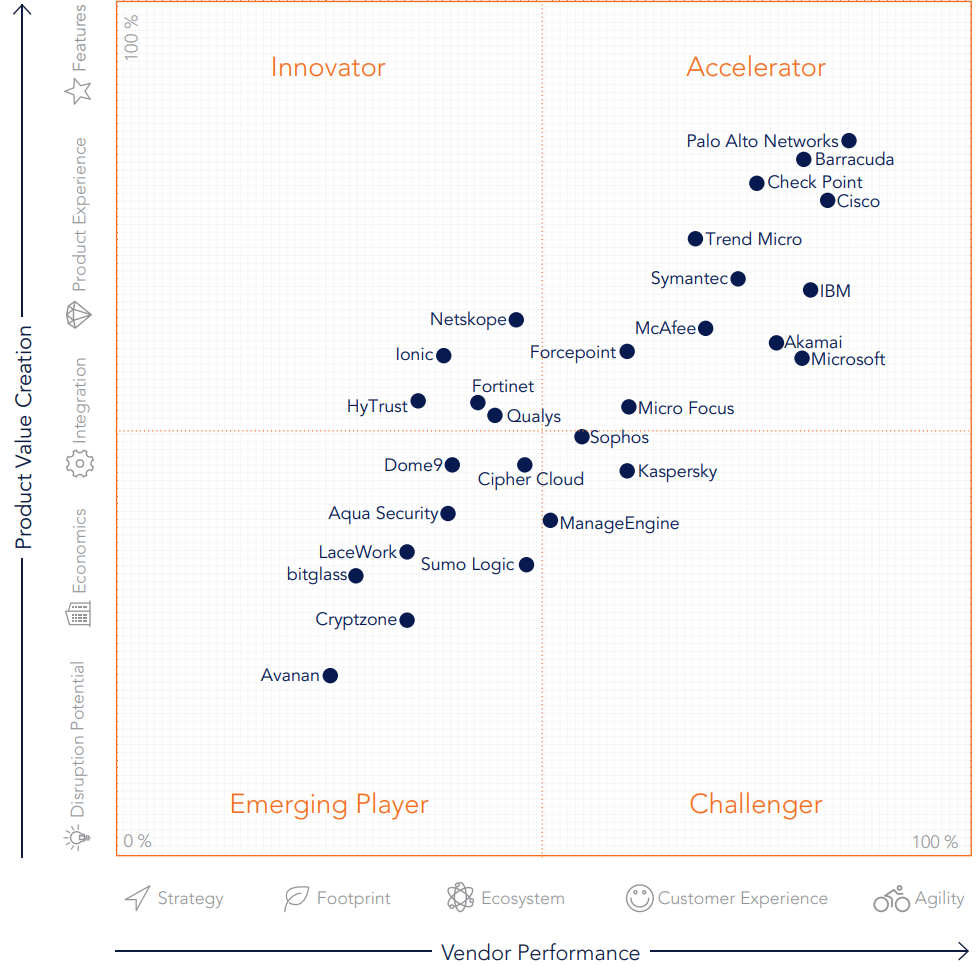
\includegraphics[width=0.8\textwidth]{img/netskopeinnovator.png}
%     \caption{ \autocite{Hille2018}}
%     \label{fig:netskope}
% \end{figure}